\documentclass[12pt,letterpaper]{report}
\usepackage{graphicx}
\usepackage{scrextend}
\usepackage{vmargin}
\usepackage[utf8]{inputenc}
\usepackage[spanish]{babel}
\usepackage{multicol}
\usepackage{amsmath, amsthm, amssymb, amsfonts}
\usepackage[usenames]{color}
\usepackage[breaklinks=true]{hyperref}
\usepackage{float}
\parindent=0mm
\pagestyle{empty}
\begin{document}
\setmargins{2.5cm}      
{1.5cm}                     
{2cm}  
{24cm}                    
{10pt}                          
{1cm}                          
{0pt}                             
{2cm} 
\begin{titlepage}
\begin{center}

\includegraphics[scale=0.40]{images/uanl.png} 
\hspace{2.5cm}

\includegraphics[scale=0.40]{images/fcfm.png}
\end{center}
\vspace{4cm}
\begin{center}
\textbf{
UNIVERSIDAD AUTÓNOMA DE NUEVO LEÓN\\
FACULTAD DE CIENCIAS FÍSICO MATEMÁTICAS\\}
\vspace*{2cm}
\begin{large}
\vspace{1cm}
\large{\textbf{Instalaci\'on necesaria para el \\Taller de Introducci\'on a la Computaci\'on Cu\'antica}}\\
\end{large}
\end{center}
\vspace{10cm}
\begin{flushright}
\today
\end{flushright}
\end{titlepage}
\section*{Windows}
\subsection*{Opci\'on 1 - Instalacion manual}
\begin{enumerate}
    \item Entra al siguiente link para descargar Python 3.x \\
    \href{https://www.python.org/downloads/release/python-385/}{Descargar python 3.x}
    \item Al momento de realizar la instalaci\'on lee muy bien las opciones que te da, ya que en algun momento te pregunta si quieres a\~nadir al PATH python, esta opci\'on debe estar habilitada.
    \item Al termino de la instalaci\'on escribe en la terminal o CMD la palabra python o python3, si no te aparece como en la figura \ref{python-terminal}, este no se encuentra en el PATH, por que lo que tendras que desinstalarlo y asegurarte que la opci\'on se encuentra habilitada.
    \begin{figure}[H]
        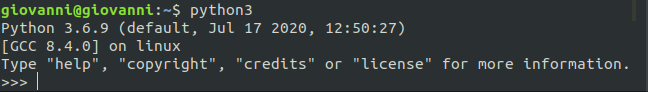
\includegraphics[scale=0.7]{images/python-print.png}
        \caption{Python abierto dentro de la terminal}
        \label{python-terminal}
    \end{figure}
    \item Despu\'es que python te aparezca en la terminal ingresa el siguiente comando para la instalaci\'on de jupyter.\\
    \textit{pip install jupyter o pip3 install jupyter} .Ojo, esto fuera de python, como si no hubieras introducido el comando python o python3.
    \item Para saber si tenemos instalado jupyter en nuestro sistema operativo introduce el comando \textit{jupyter notebook o jupyter-notebook}, y te debera de aparecer como en la figura \ref{jupyter}
    \begin{figure}[H]
        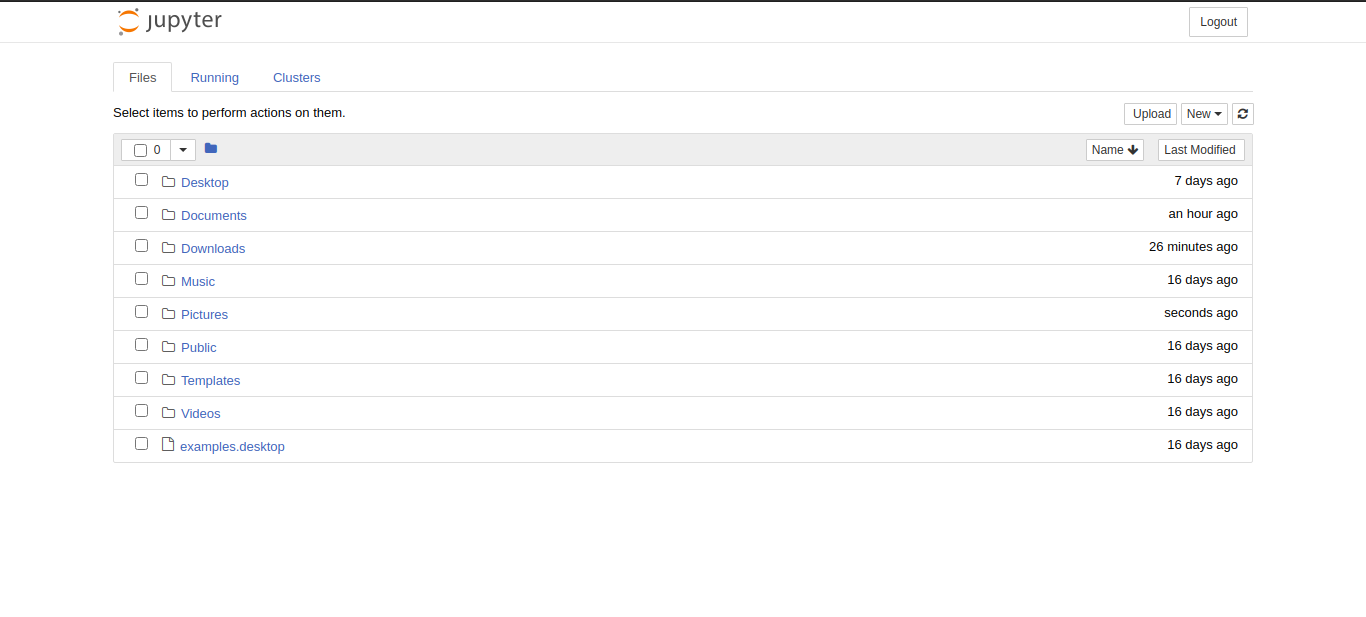
\includegraphics[scale=0.3]{images/jupyter.png}
        \caption{Jupyter}
        \label{jupyter}
    \end{figure}
    \item Ya con esto solo quedara instalar las siguiente librerias de python con los siguientes comandos\\
    \textit{pip install numpy\\
    pip install matplotlib\\
    pip install scipy\\
    pip install qiskit\\}
    si no te funcionan estos comandos en ves de pip intenta con pip3
\end{enumerate}
\subsection*{Opci\'on 2}
Se puede realizar la instalaci\'on de anaconda pero no lo recomiendo porque pueden existir problemas de compatibilidad y es m\'as complicado resolverlos. De todas formas si decides este camino no tienes que instalar todo, con que instales anaconda el unico comando que te faltara es el siguiente:\\
\textit{pip install qiskit}\\
esto en la terminal de comandos de anaconda
\section*{Ubuntu/Unix}
\subsection*{Opci\'on 1 - Instalacion manual}
\begin{enumerate}
    \item En linux/unix no tienes que instalar python, ya esta por defecto, solo que tendras que usar el comando python3 para que estes usando python 3.x, ya que el sistema puede contener la version 2.x, la manera en la cual debera aparecerte es como en la figura \ref{python-terminal2}
    \begin{figure}[H]
        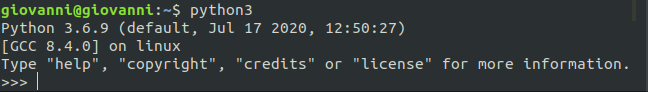
\includegraphics[scale=0.7]{images/python-print.png}
        \caption{Python abierto dentro de la terminal}
        \label{python-terminal2}
    \end{figure}
    \item Despu\'es que python te aparezca en la terminal ingresa el siguiente comando para la instalaci\'on de jupyter.\\
    \textit{sudo apt install jupyter-notebook} .Ojo, esto fuera de python, como si no hubieras introducido el comando python o python3.
    \item Para saber si tenemos instalado jupyter en nuestro sistema operativo introduce el comando \textit{jupyter notebook o jupyter-notebook}, y te debera de aparecer como en la figura \ref{jupyter-linux}
    \begin{figure}[H]
        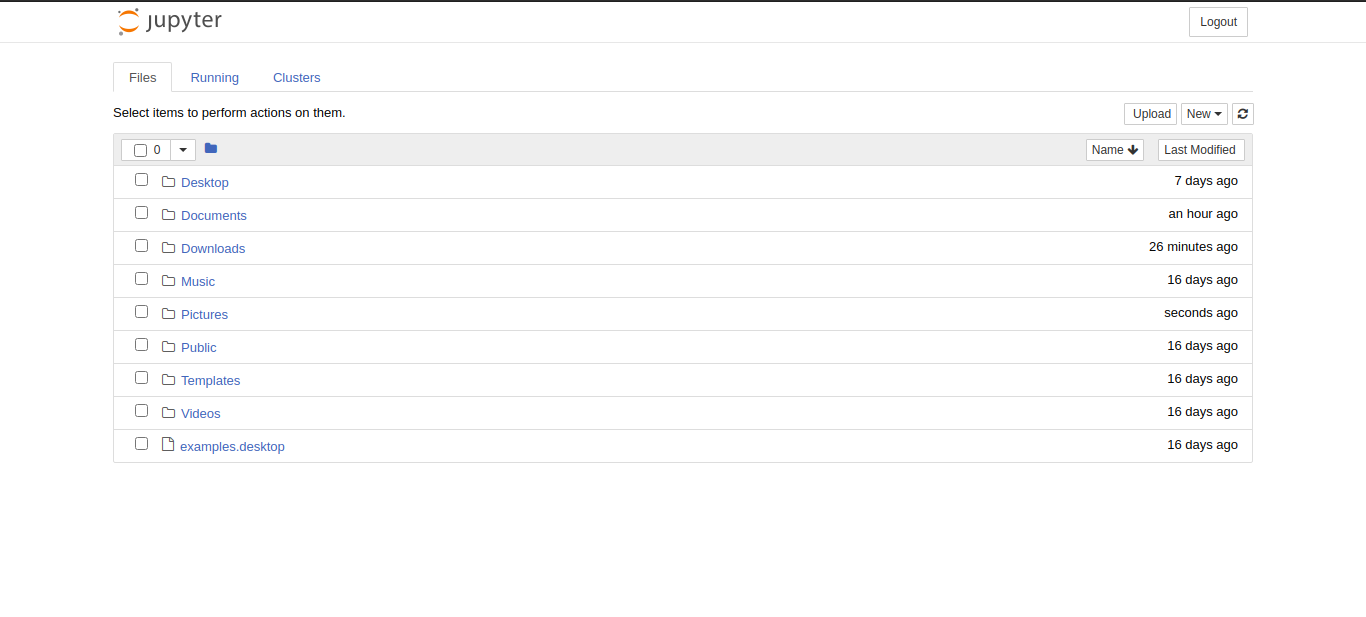
\includegraphics[scale=0.3]{images/jupyter.png}
        \caption{Jupyter}
        \label{jupyter-linux}
    \end{figure}
    \item Ya con esto solo quedara instalar las siguiente librerias de python con los siguientes comandos\\
    \textit{pip install numpy\\
    pip install matplotlib\\
    pip install scipy\\
    pip install qiskit\\}
    si no te funcionan estos comandos en ves de pip intenta con pip3
\end{enumerate}
\subsection*{Opci\'on 2}
Se puede realizar la instalaci\'on de anaconda pero no lo recomiendo porque pueden existir problemas de compatibilidad y es m\'as complicado resolverlos. De todas formas si decides este camino no tienes que instalar todo, con que instales anaconda el unico comando que te faltara es el siguiente:\\
\textit{pip install qiskit}\\
\end{document}